\documentclass[12pt]{article}
\usepackage[a4paper, total={6in, 9in}]{geometry}
\usepackage{graphicx}
\graphicspath{ {./images/output/} }
\usepackage{caption}
\usepackage[english]{babel}
\usepackage{titling}
\usepackage{float}
% \usepackage{amsmath}
% \usepackage{minted}
% \usepackage{multicol}
% \usepackage{array}
% \usepackage{setspace}
% \usepackage{placeins}

% \usepackage{lipsum}

\title{Study of Buck Converter Using Simulink}
\author{}
\date{}

\pagenumbering{gobble}
\begin{document}
\vspace*{\fill}
\begin{center}

    \emph{Heaven's Light is Our Guide} \\
    \textbf{Rajshahi University of Engineering and Technology} \\

    \begin{figure}[H]
        \centering
        
\includegraphics[scale=.34]{images/RUET_logo.png}
        \label{fig:ruet_logo}
    \end{figure}
    \vspace{5mm}

    \textbf{Course Code}\\
    ECE 3206\\
    \vspace{3mm}
    \textbf{Course Title}\\
    Industrial Electronics Sessional

    \vspace{5mm}
    \textbf{Experiment Date:} {January 13, 2025},\\
    \textbf{Submission Date:} {February 10, 2025}\\

    \vspace{5mm}
    \textbf{Lab Report 3: \\
        Study of Thyristor Characteristics R, RL Load}

    \vspace{15mm}

    \begin{tabular}{c|c}
        \textbf{Submitted to} & \textbf{Submitted by} \\
        Md. Faysal Ahamed     & Md. Tajim An Noor     \\
        Lecturer              & Roll: 2010025         \\
        Dept of ECE, Ruet     &                       \\
    \end{tabular}

\end{center}
\vspace*{\fill}


\pagebreak

\tableofcontents

\pagebreak
\pagenumbering{arabic}
\maketitle

\section*{Working Principle of Boost Converter}
\addcontentsline{toc}{section}{Working Principle of Boost Converter}
A DC-DC Boost Converter (Step-Up Chopper) is a type of SMPS that increases input DC voltage to a higher output DC voltage using high-speed switching devices.

\subsection*{Circuit Diagrams}
\begin{figure}[H]
    \centering
    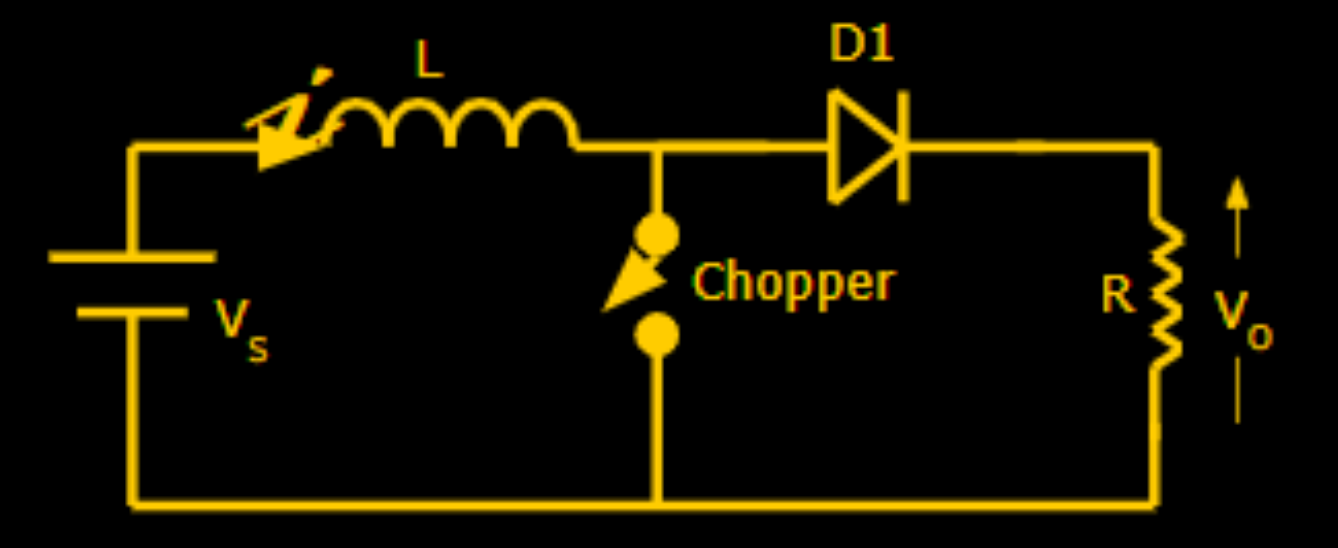
\includegraphics[width=.5\textwidth]{ckt.png}
    \caption{Basic Circuit Diagram of a DC-DC step up Circuit}
\end{figure}

\subsection*{Key Components}
The key components of a boost converter include:
\begin{itemize}
    \item An inductor (L)
    \item A switch (typically a MOSFET or IGBT)
    \item A diode (D)
    \item A filter capacitor (C)
    \item A load resistance (R)
\end{itemize}

\subsection*{Operation Modes}
The operation of a boost converter consists of two intervals in each switching cycle:
\begin{description}
    \item \textbf{ON-State (Switch Closed, $t_1$):}
          \begin{itemize}
              \item The switch is ON, and current flows from the source $(V_s)$ through the inductor, storing energy as a magnetic field.
              \item The diode is reverse-biased, blocking current to the load.
              \item Inductor voltage: \( V_L = V_s \), and current increases linearly: \( \frac{di}{dt} = \frac{V_s}{L} \).
          \end{itemize}
    \item \textbf{OFF-State (Switch Open, $t_2$):}
          \begin{itemize}
              \item The switch is OFF, and the inductor releases stored energy.
              \item Current flows through the diode, charging the capacitor and powering the load.
              \item Output voltage: \( V_O = V_S + V_L \), higher than the input.
          \end{itemize}
\end{description}
This cyclical switching process results in a higher average output voltage.

\subsection*{Output Voltage Expression}
\begin{figure}[H]
    \centering
    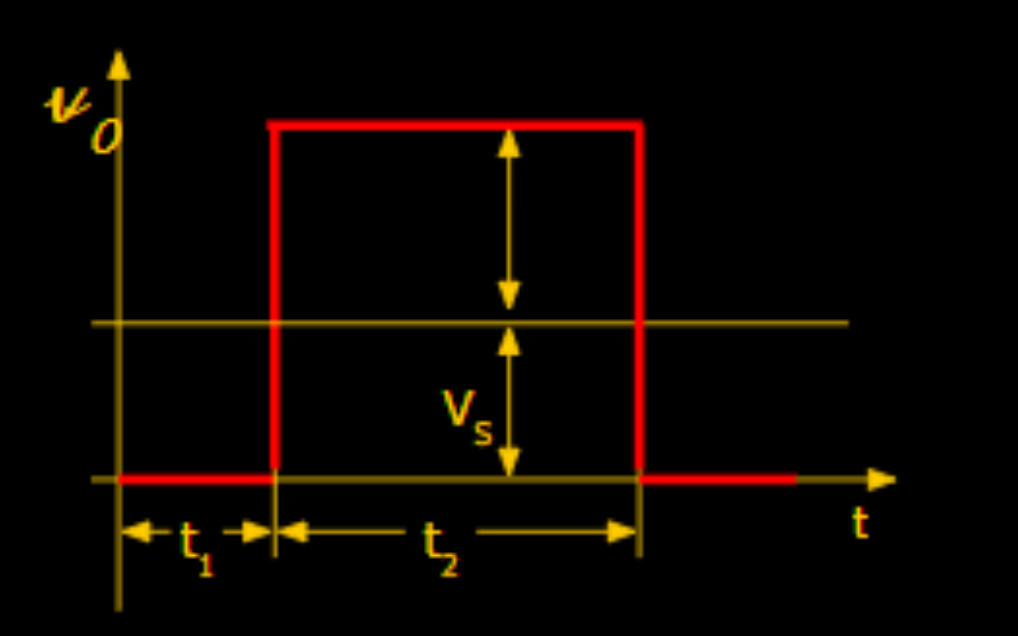
\includegraphics[width=.5\textwidth]{ch1.png}
    \caption{Output Voltage of the Booster Circuit}
\end{figure}

The output voltage of a boost converter is related to the input voltage and the duty cycle \( K \) by
the following equation:
\[
    V_O = \frac{V_S}{1 - K}
\]
Where:
\begin{itemize}
    \item \( V_O \) = Output Voltage
    \item \( V_S \) = Input Voltage
    \item \( K = \frac{t_1}{T} \) = Duty cycle (ratio of ON time to total period)
\end{itemize}
As \( K \) approaches 1 (i.e., longer ON-time), the output voltage increases significantly. However, it
can never be infinite due to practical limitations such as switch losses and component ratings.\cite{lm2577t-adj}

\subsection*{Current Behavior}
\begin{figure}[H]
    \centering
    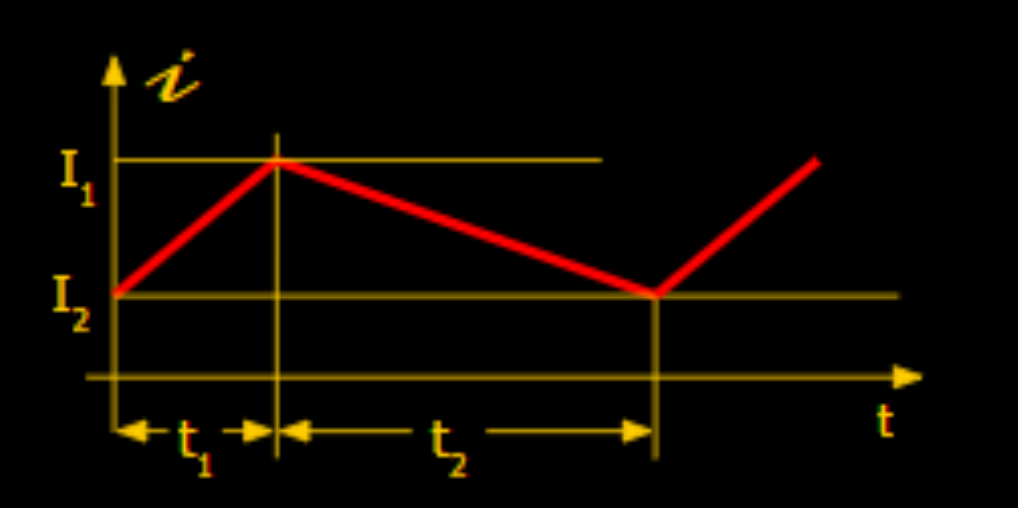
\includegraphics[width=.5\textwidth]{ch2.png}
    \caption{Output Current of the Booster Circuit}
\end{figure}
The inductor current forms a triangular waveform, ramping up during the ON state and down during the OFF state. Proper inductance and switching frequency minimize ripple.\cite{lm2577t-adj}

\section*{Designing a DC-DC Boost Converter:}
\addcontentsline{toc}{section}{Designing a DC-DC Boost Converter:}
\subsection*{Necessary Components}
\begin{itemize}
    \item LM2577T – Adjustable IC (1 piece)
    \item 100 µH Inductor (1 piece)
    \item IN5819 Schottky Diode (1 piece)
    \item 2k$\Omega$ Resistor (2 pieces)
    \item 220$\Omega$ Resistor (1 piece)
    \item Red LED (1 piece)
    \item 10µF Capacitor (1 piece)
    \item 470µF Capacitor (1 piece)
    \item 330nF Capacitor (1 piece)
    \item Trimmer/Variable Potentiometer 100k (1 piece)
    \item Screw Terminal (2 pieces)
    \item Slide Switch (1 piece)
    \item 5x1 Female Header Pin (1 piece)
    \item 5x1 Male Header Pin (1 piece)
    \item Digital Voltmeter + Ammeter (1 piece)
    \item Soldering Iron
    \item Solder
    \item Multimeter
\end{itemize}
\subsection*{Necessary Software:}
\begin{itemize}
    \item EasyEDA for Circuit Diagram and PCB Designing
\end{itemize}

\subsection*{Components choosing Justification:}
\begin{description}
    \item \textbf{LM2577-ADJ:} A versatile boost converter IC with integrated switch, oscillator, and feedback control, allowing adjustable output voltage via external resistors.
    \item \textbf{IN5819 (Schottky Diode):} Chosen for its low forward voltage drop and fast recovery, ensuring efficient high-frequency switching with minimal losses.
    \item \textbf{100 µH Inductor:} Stores and releases energy during switching, enabling voltage boost while minimizing current ripple.
    \item \textbf{330 pF Capacitor:} Stabilizes the LM2577's feedback loop for smooth output regulation.
    \item \textbf{470 µF Capacitor:} Filters and smooths the boosted DC output, reducing ripple and transients.
    \item \textbf{100k$\Omega$ Potentiometer:} Adjusts output voltage by forming a feedback voltage divider with R1.
    \item \textbf{2k$\Omega$ Resistor:} Works with the potentiometer to set the feedback ratio and stabilize the output voltage.
\end{description}

\subsection*{Circuit Diagram}
The circuit diagram illustrates a DC-DC boost converter using the LM2577-ADJ IC to step up a 5V input. Key components include a 100 µH inductor, 1N5819 Schottky diode, and adjustable potentiometer for output voltage control. Screw terminals and header pins ensure secure connections, while capacitors provide filtering and stability.
\begin{figure}[H]
    \centering
    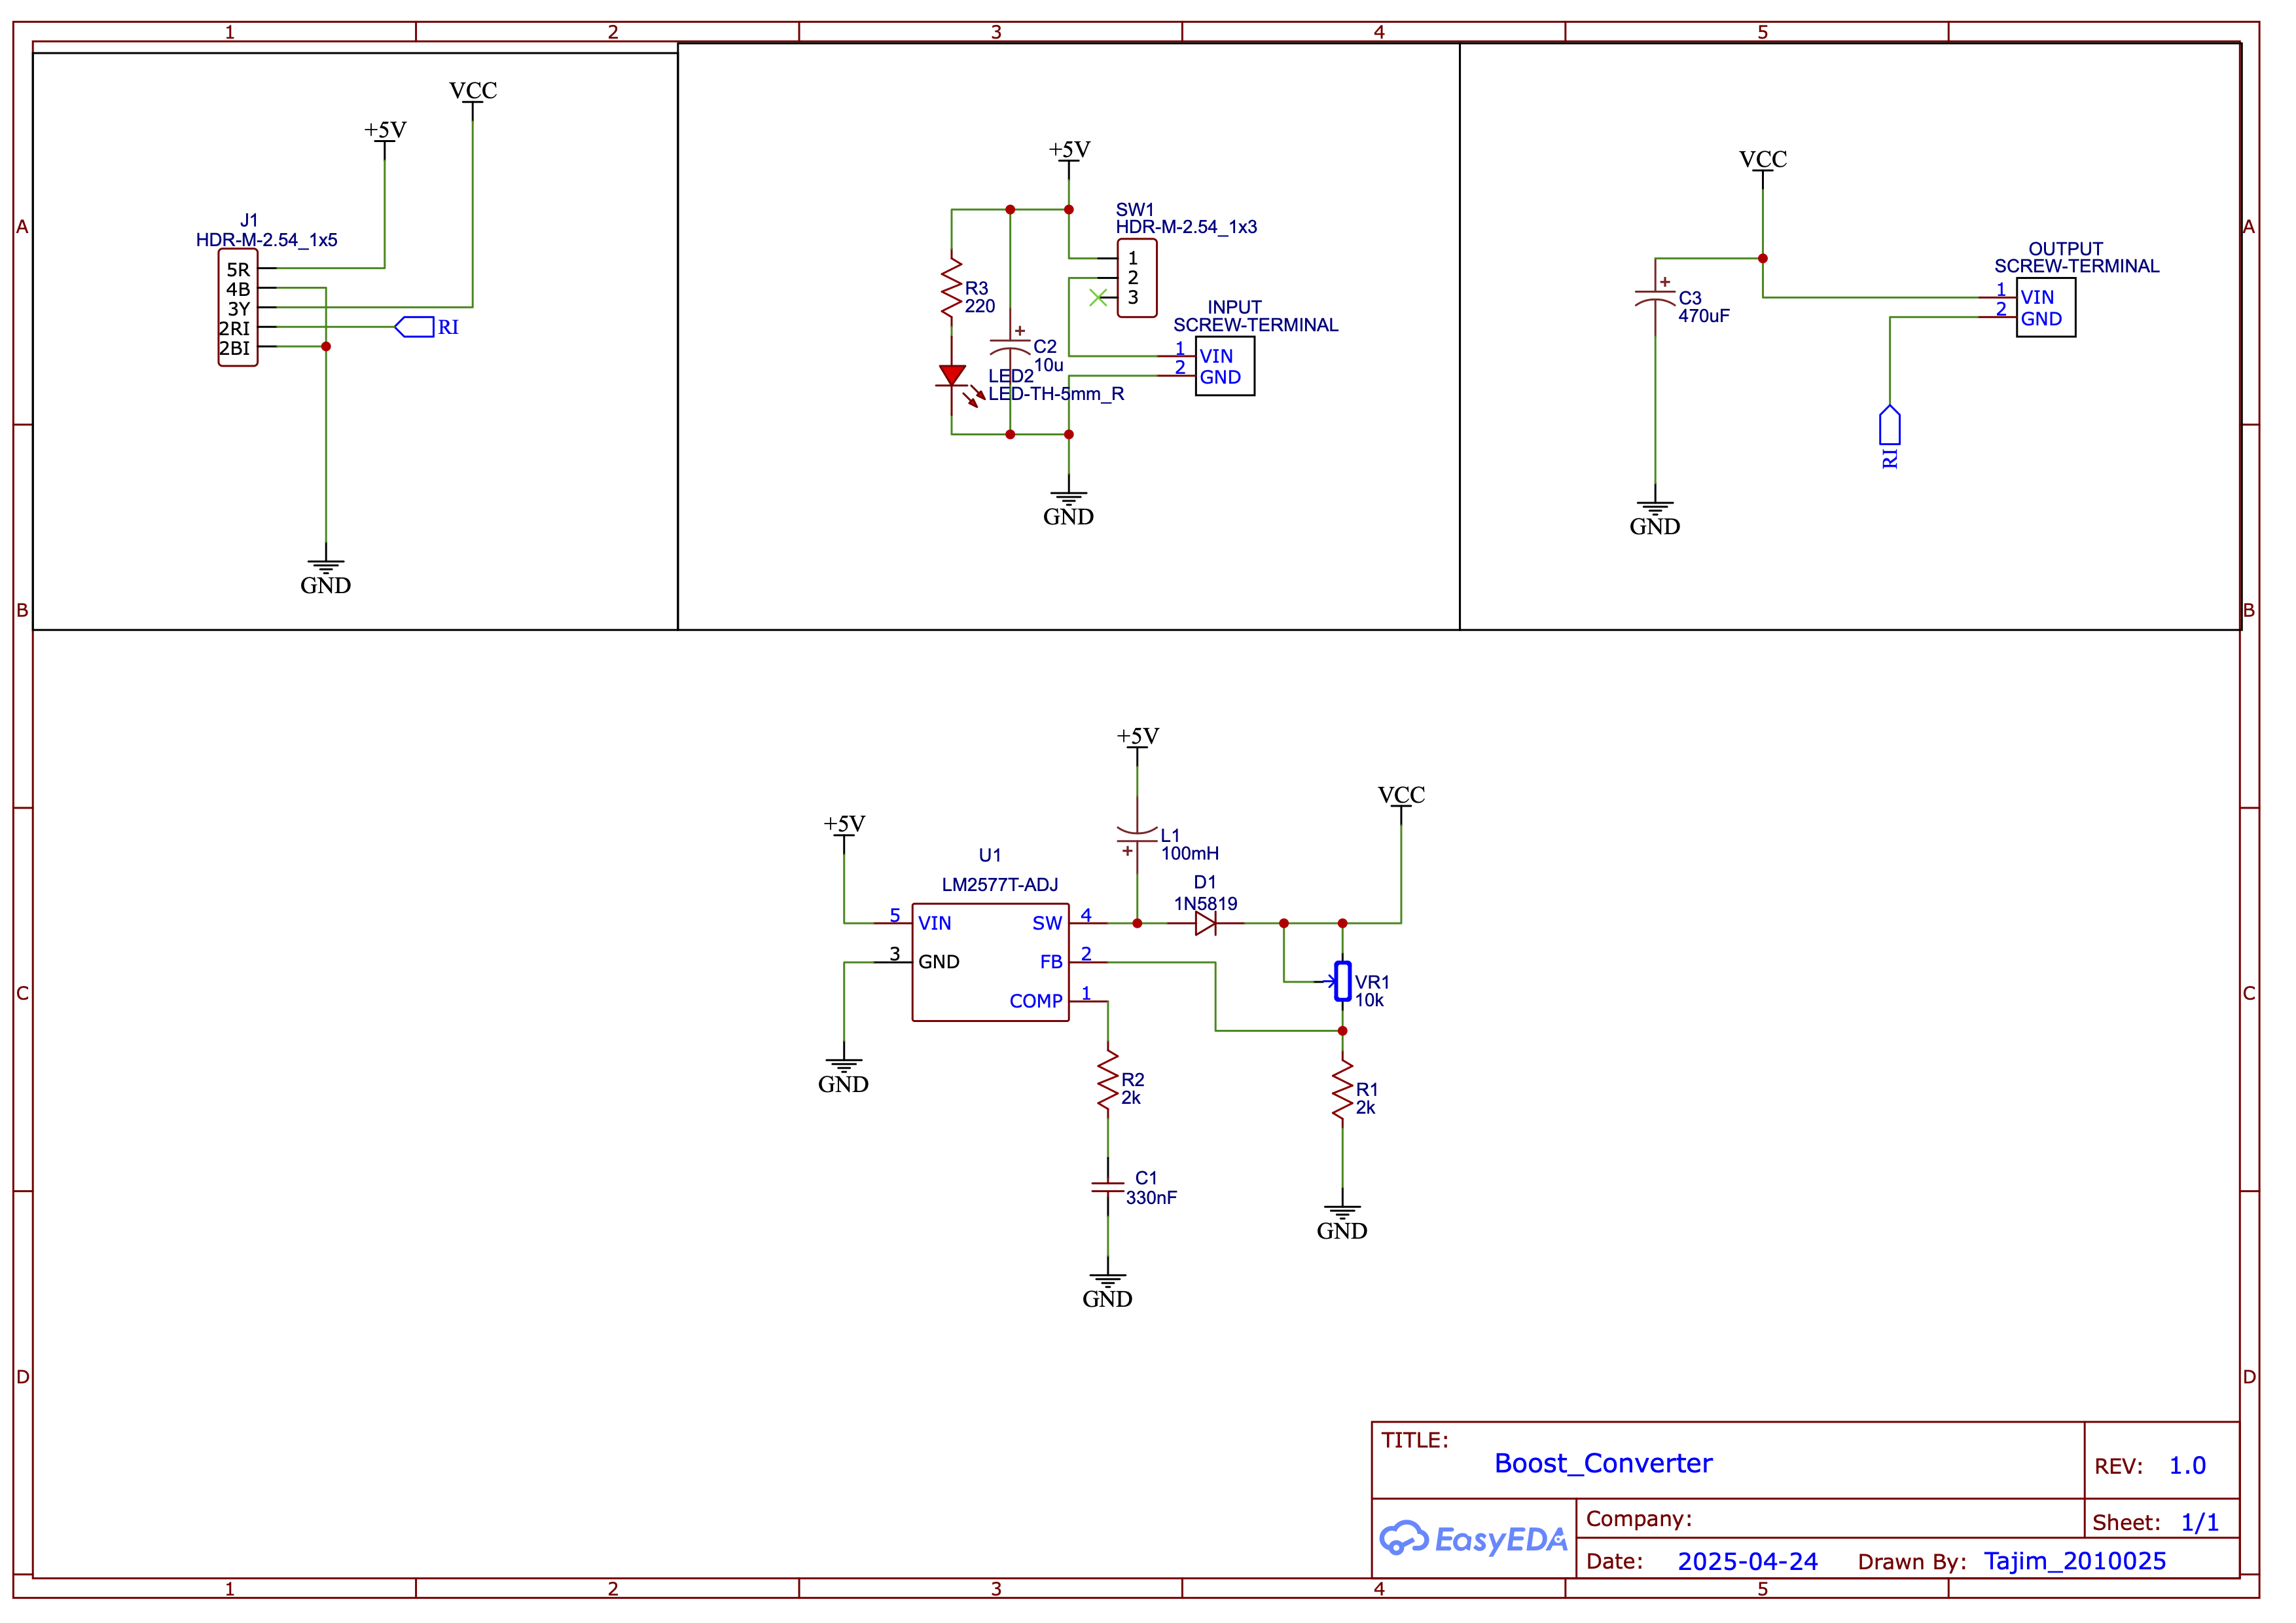
\includegraphics[width=\textwidth]{booCon.png}
    \caption{Precise Circuit Diagram of DC-DC booster Circuit}
    \label{fig:rControlledNoDelay}
\end{figure}

\subsection*{Printed Circuit Board (PCB) and 3D rendered View:}
\begin{itemize}
    \item PCB layout was designed with proper placement of components like LM2577 IC, inductor, and Schottky diode.
    \item Tracks were optimized for short, efficient high-current paths and ground planes added for noise reduction.
    \item Mounting holes and labels were included for easy assembly, and a DRC ensured error-free design.
\end{itemize}

\begin{figure}[H]
    \centering
    \begin{minipage}{0.48\textwidth}
        \centering
        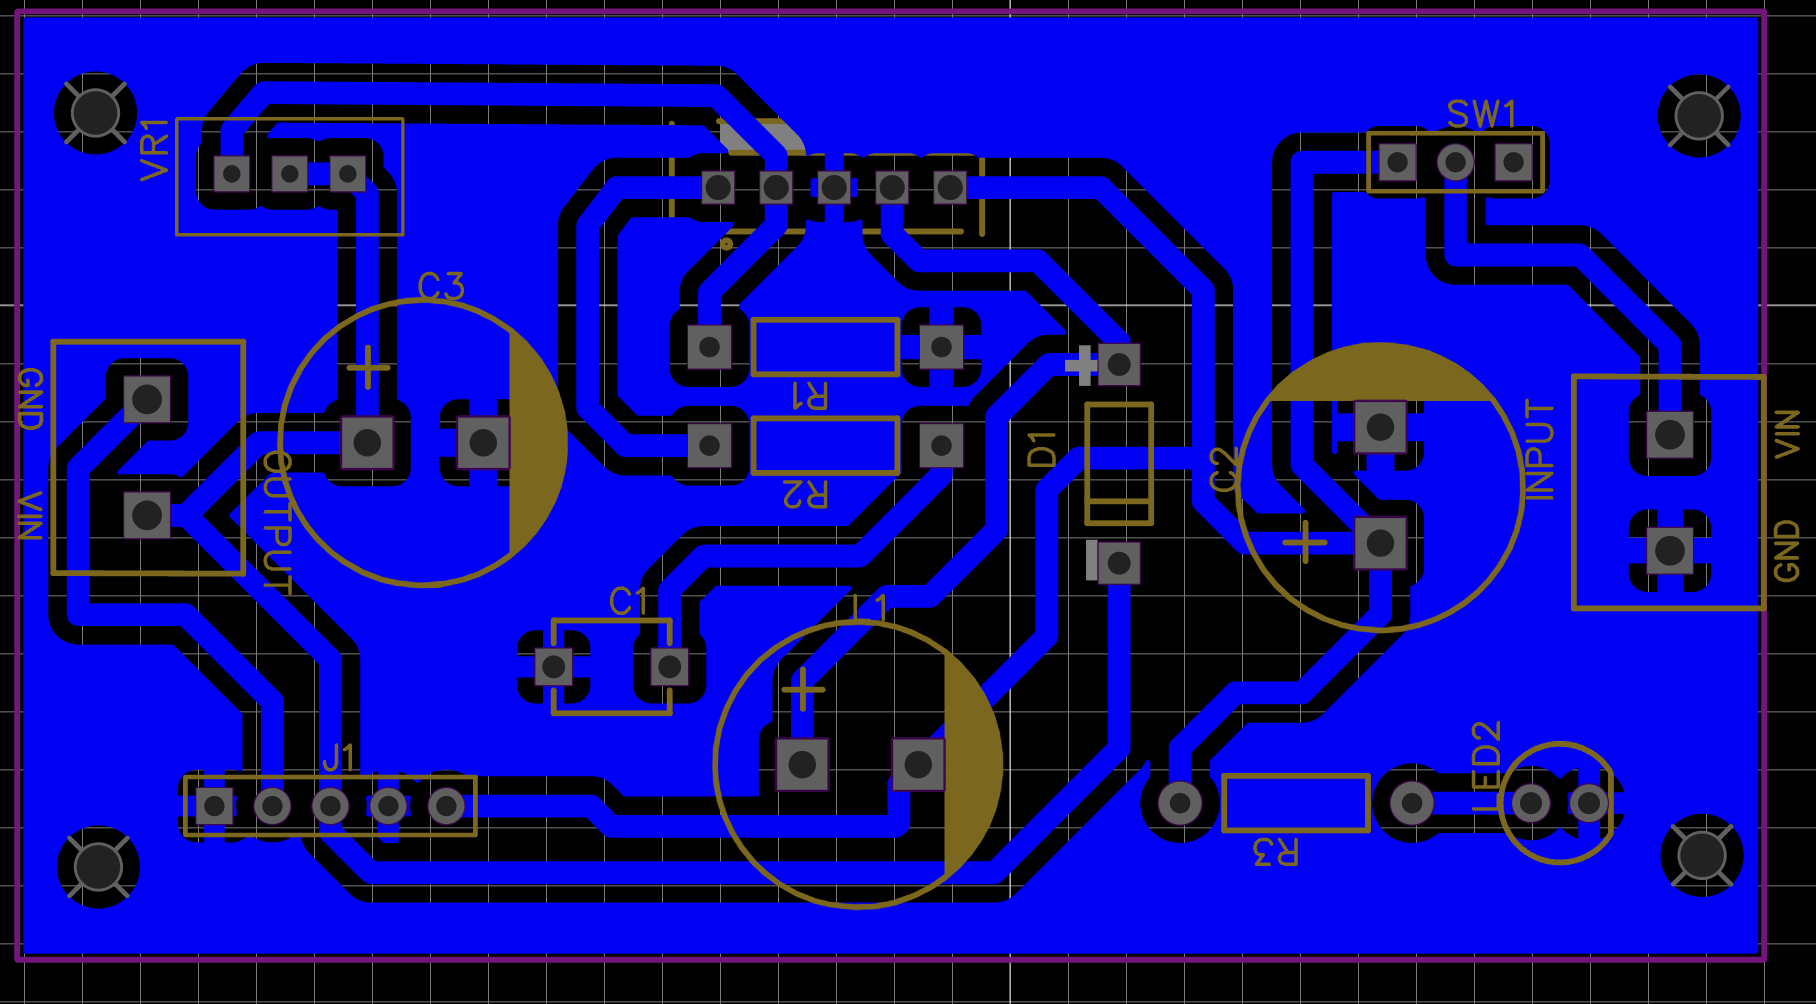
\includegraphics[width=\textwidth]{pcb.png}
        \caption{PCB Design}
    \end{minipage}
    \hfill
    \begin{minipage}{0.48\textwidth}
        \centering
        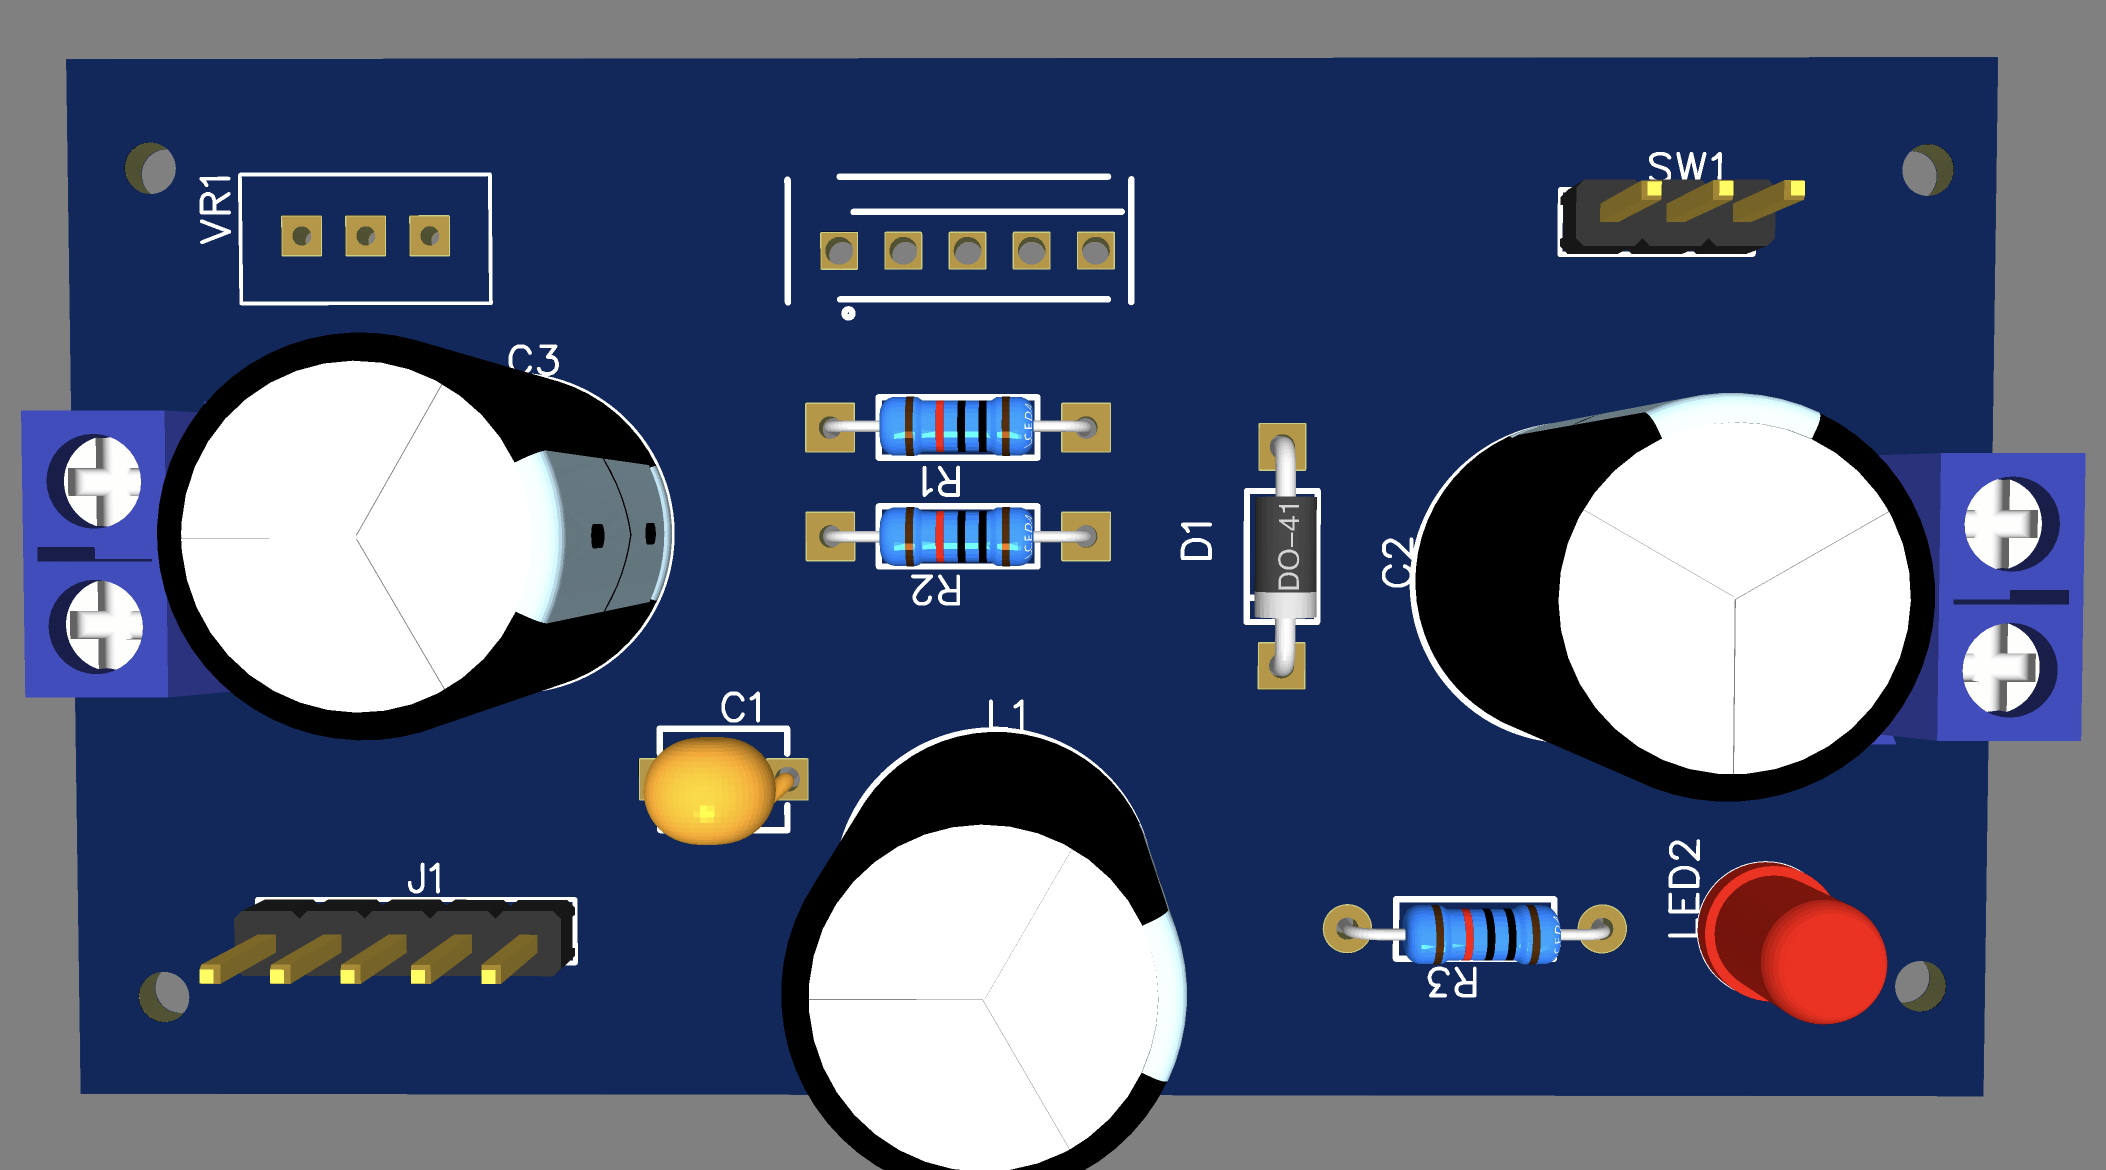
\includegraphics[width=\textwidth]{3d.png}
        \caption{3D Rendered View of PCB}
    \end{minipage}
\end{figure}


\subsection*{Input-Output of the DC-DC Step Up Circuit:}
According to the data sheet of the LM 2577,
Voltage Output, \( V_out = 1.23 \left( 1 \times
\frac{R_1}{VR_1} \right) \)
Where,
\( V_out \) = Output Voltage of the Step Up circuit \\
\( R_1 = 2 \, k\Omega \) \\
\( VR_1 \) = Variable Resistor of \( 100 \, k\Omega \)

\begin{figure}[H]
    \centering
    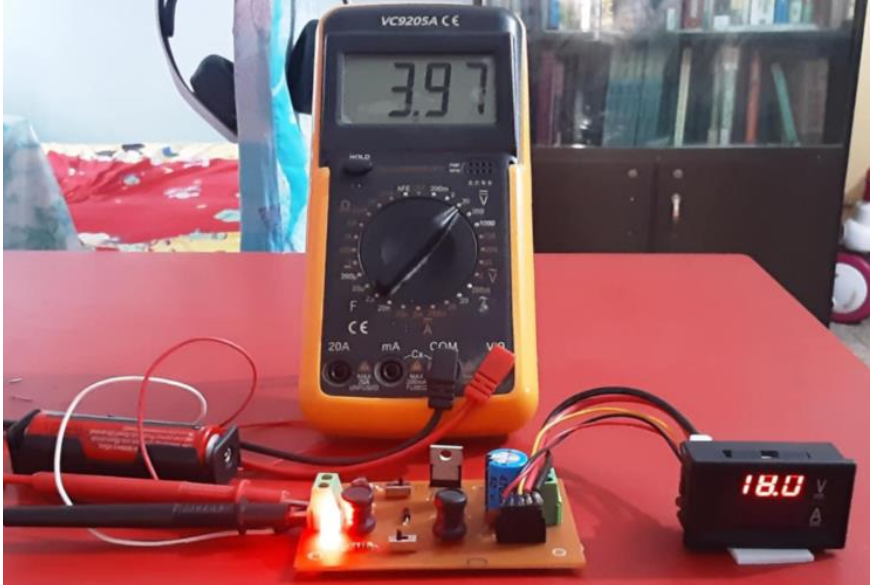
\includegraphics[width=.5\textwidth]{pr.png}
    \caption{4V input and 18V output}
\end{figure}

\section*{Result Discussion}
\addcontentsline{toc}{section}{Result Discussion}
The aim of this project was to design and build a DC-DC step-up (boost) converter using the LM2577-ADJ IC. The circuit was designed and simulated in EasyEDA, and the PCB layout was created following best practices for switching power supplies, including optimized trace routing, decoupling, and component placement. After assembling the PCB and soldering the components, the circuit was tested and verified to operate as expected.\\\\
When powered by a 3.7V lithium-polymer (LiPo) battery, the converter successfully delivered a stable adjustable output voltage ranging from approximately 8V to 72V. This wide range highlights the efficiency of the feedback control loop and the switching process. The onboard potentiometer allowed precise adjustment of the output voltage, while real-time voltage readings were monitored using an external voltmeter/ammeter module connected via header pins.\\\\
During testing, the circuit exhibited stable performance without any thermal or functional issues. The use of a 1N5819 Schottky diode reduced switching losses, and the careful component layout minimized electromagnetic interference (EMI). Additionally, the power indicator LED and output filtering capacitors improved usability and ensured a smooth output voltage.

\section*{Applications of DC-DC Boost Converter}
\addcontentsline{toc}{section}{Applications of DC-DC Boost Converter}
\begin{itemize}
    \item DC motor drive systems
    \item Electric vehicles
    \item Battery voltage regulators
    \item Solar photovoltaic systems
    \item Regenerative braking in traction systems
\end{itemize}

\section*{Conclusion}
\addcontentsline{toc}{section}{Conclusion}
The boost converter is an efficient solution for stepping up DC voltage through a switching mechanism. By controlling the switch's duty cycle, the output voltage can be effectively regulated. Mastering its operation is crucial in power electronics, especially for developing efficient power conversion applications.

\bibliographystyle{IEEEtran}
\renewcommand{\bibname}{References}
\addcontentsline{toc}{section}{References}
\bibliography{ref}

\end{document}
